\documentclass[../master]{subfiles}

\begin{document}
\chapter{ドリフトスピード}
\section{水分のドリフトスピードへの影響}
本研究では用いた検出ガスは低圧であるため,
水分などの不純物からの影響が大きいと考えられる.
そこで,チェンバー中の水分をモニターしながらドリフトスピードの変化を測定した.
水分は露点計で測定した.
露点温度と水分濃度と蒸気密度の対応を表\ref{tab::dew_point_humidity}に示す.
\begin{table}
  \centering
  \caption{露点温度と水分濃度と蒸気密度の対応.ppmはparts par millionの略であり, 10,000 ppm = 1\% となる.}
  \label{tab::dew_point_humidity}
  \begin{tabular}{ccc}
    \toprule
    露点温度 \si{\degreeCelsius} & 水分濃度 (ppm) & 蒸気密度 \si{\gram/\cubic\metre} \\
    \midrule
    $-80$ & 0.540 & 0.000613 \\
    $-70$ & 2.581 & 0.00279 \\
    $-60$ & 10.67 & 0.0109 \\
    $-50$ & 38.84 & 0.0382 \\
    $-40$ & 126.7 & 0.1199 \\
    $-30$ & 375.0 & 0.339 \\
    $-20$ & 1019 & 0.884 \\
    $-10$ & 2565 & 2.14 \\
    0     & 6032 & 4.85 \\
    \bottomrule
  \end{tabular}
\end{table}

\begin{figure}
  \centering
  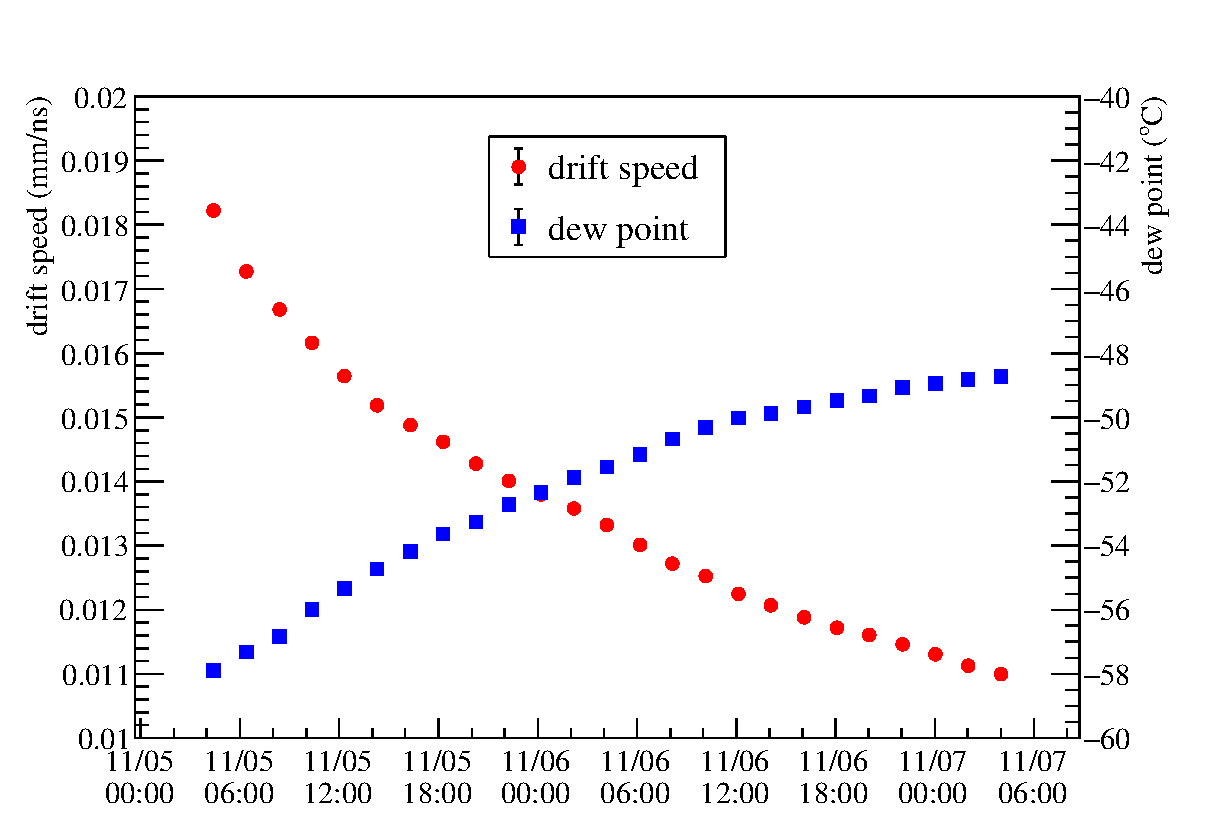
\includegraphics[clip, width=0.8\columnwidth]{drift_time_dep.eps}
  \caption{ドリフトスピードと露点温度の時間変化.}
  \label{fig::drift_time_dep}
  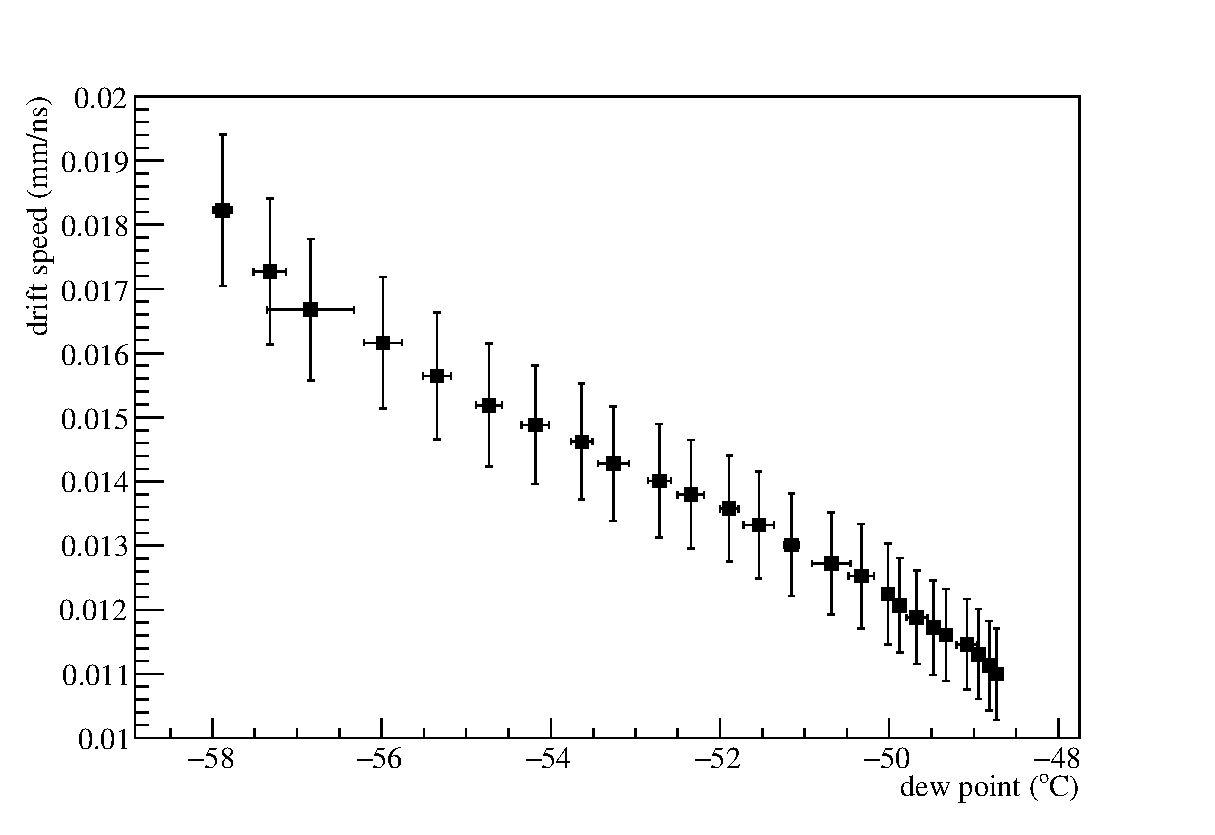
\includegraphics[clip, width=0.8\columnwidth]{drift_dew_dep.eps}
  \caption{ドリフトスピードの露点温度依存性.}
  \label{fig::drift_dew_dep}
\end{figure}

\end{document}
